\documentclass[letterpaper]{article}
\usepackage[utf8]{inputenc}
\usepackage[spanish]{babel}
\usepackage{amssymb, amsmath}
\usepackage{stackengine}
\usepackage{graphicx}
\usepackage{ mathrsfs }
\usepackage{lipsum}
\usepackage{dsfont}
\usepackage[margin=1.5cm,
vmargin={1.5cm,0.7cm},
includefoot]{geometry}
\usepackage{setspace}
\usepackage{subcaption}
\usepackage{tocloft}
\usepackage{upgreek}
\usepackage{amsthm}
\usepackage{graphicx}
\usepackage{paralist}
\usepackage{fancyhdr}
\usepackage{lmodern}
\usepackage{tcolorbox}
\usepackage{color}
\usepackage{tikz}
\usepackage{wasysym}
\usepackage{textgreek, marvosym}
\tcbuselibrary{skins,breakable}
\pagestyle{fancy}

\renewcommand{\headrulewidth}{0.4pt}
\renewcommand{\footrulewidth}{0.4pt}

\renewcommand{\d}{\partial}

\providecommand{\abs}[1]{\left|#1\right|}
\providecommand{\norm}[1]{\left|\left|#1\right|\right|}														  
\providecommand{\pint}[1]{\langle#1\rangle}														  
\newcommand{\V}{\mathds{V}}

\newcommand{\W}{\mathds{W}}

\newcommand{\F}{\mathds{F}}

\newcommand{\tq}{ \quad \cdot  \backepsilon \cdot \quad }

\newcommand{\ld}{\lim\limits_{x \to 0^{+}}}

\newcommand{\li}{\lim\limits_{x \to 0^{-}}}

\newcommand{\la}{\lim\limits_{x \to a}}

\renewcommand{\l}{\ell}

\newcommand{\R}{\mathds{R}}

\newcommand{\Po}{\mathds{P}_2(\mathds{R})}

\renewcommand{\*}{\cdot}

\newcommand{\Iden}{\begin{pmatrix}
		1 & 0 & 0\\
		0 & 1 & 0\\
		0 & 0 & 1 
\end{pmatrix}}
\newcommand{\T}{\begin{pmatrix}
		1 & 3 & 9 \\
		1 & 3 & 4 \\
		0 & 0 & 2 
\end{pmatrix} }

\makeatletter
\renewcommand*\env@matrix[1][\arraystretch]{%
	\edef\arraystretch{#1}%
	\hskip -\arraycolsep
	\let\@ifnextchar\new@ifnextchar
	\array{*\c@MaxMatrixCols c}}
\makeatother

\newtheorem{theorem}{Teorema}[]
\theoremstyle{definition}
\newtheorem{definition}{Definición}


\begin{document}
	
	\setlength{\unitlength}{1cm}
	\thispagestyle{empty}
	\begin{picture}(19,3)
	\put(-0.5,1.2){
\includegraphics[scale=.20]{img/unam1.png}}
	\put(16,1){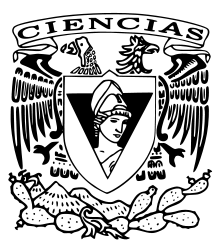
\includegraphics[scale=.29]{img/fciencias1.png}}
	\end{picture}
	
	\begin{center}
		\vspace{-114pt}
		\textbf{\large Matemáticas para las Ciencias II}\\
		\textbf{ Semestre 2020-2}\\
		Prof. Pedro Porras Flores\\
		Ayud. Irving Hernández Rosas \\
		\textbf{Proyecto V}\\[0.2cm]
		Kevin Ariel Merino Peña\footnote{Número de cuenta 317031326}\\ [0.2cm]
	\end{center}
	\vspace{-10pt}
	\rule{19cm}{0.3mm}
	
\noindent Realice los siguientes ejercicios, escribiendo el procedimiento claramente. Y recuerden que estos proyectos se entregan de manera individual en la plataforma de google classroom.\\


\noindent1.  Verifique el primer caso de la regla de la cadena de la composición $ f\circ \vec{\gamma}$ para cada uno de los siguientes casos, esto es primero haga la composición y derive, y le luego use la regla de la cadena y vea que se llega al mismo resultado.\\
\begin{theorem}[Regla de la cadena]
	\relax
	Sean $ U\subset \R^n $ y $ V \subset \R^m $ conjuntos abiertos, $ g: U \subset \R^n \to \R^m $ y $ f: V\subset \R^m \to \R^p $ dos funciones tales que $ g $ manda a $ U $ en $ V $ \textit{i.e. } $ f \circ g $. Supogamos que $ g $ es diferenciable en $ \vec{x_0} $ y $ D(f \circ g) (\vec{x_0}) = Df(g(\vec{x_0}))Dg(\vec{x_0}) $.\\
	\begin{itemize}
		\item \textbf{Primer caso de la regla de la cadena}\\
		
		Supongamos $ \vec{\gamma}: \R \to \R^3 $ es una trayectoria diferenciable y $ f: \R^3 \to \R $. Sea $ h(t) = f(\vec{\gamma})(t) = f(x(t), y(t), z(t)  $ donde 
		$ \vec{\gamma}(t)= (x(t),y(t),z(t)) $. Entonces
		\[  \dfrac{dh}{dt} = \dfrac{\d f}{\d x} \dfrac{dx}{dt} +  \dfrac{\d f}{\d y} \dfrac{dy}{dt} +  \dfrac{\d f}{\d z} \dfrac{dz}{dt} \]
		esto es:
		\[ \dfrac{dh}{dt} = \nabla f(\gamma(t)) \* \vec{\gamma'}(t) \] donde $ \vec{\gamma'}(t)= (x'(t),y'(t),z'(t))  $.
		
		\item  \textbf{Segundo caso de la regla de la cadena }\\
		
		Sean $ f:\R^3 \to \R $ y $ g:\R^3 \to \R^3 $. Escribimos 
		\[ g(x,y,z) = (u(x,y,x), v(x,y,z), w(x,y,z) \quad \text{  y  }\quad h(x,y,z) = f(u(x,y,z), u(x,y,z), w(x,y,z))  \]
		Entonces:
	\[ \begin{pmatrix}
	\dfrac{\d h}{\d x} & \dfrac{\d h}{\d y} & \dfrac{\d h}{\d x}
	\end{pmatrix} = \begin{pmatrix}
	\dfrac{\d f}{\d x} & \dfrac{\d f}{\d y} & \dfrac{\d f}{\d z}
	\end{pmatrix} \begin{pmatrix}[2]
	\dfrac{\d u}{\d x} & \dfrac{\d u}{\d x} & \dfrac{\d u}{\d x}\\
	\dfrac{\d v}{\d x} & \dfrac{\d v}{\d x} & \dfrac{\d v}{\d x}\\
	\dfrac{\d w}{\d x} & \dfrac{\d w}{\d x} & \dfrac{\d w}{\d x}\\
	\end{pmatrix} \]
	\end{itemize}
\end{theorem}

a) $f(x,y) = xy$, $\vec{\gamma}(t) =(e^t, \cos(t)) $.\\
Tenemos que $  f \circ \gamma(t) = e^t\cos(t) $ y su derivada es 
\begin{align*}
	\dfrac{d}{dt} (f\circ \gamma) &= \dfrac{d}{dt}e^t\cos(t) &&\text{Planteando la derivada}\\
	\dfrac{d}{dt} (f\circ \gamma) &= e^t\dfrac{d}{dt}\cos(t) + \cos(t)\dfrac{d}{dt}e^t &&\text{Por la regla del producto en derivadas}\\
	\dfrac{d}{dt} (f\circ \gamma) &= e^t(- \sin(t)) + \cos(t)e^t &&\text{Por nuestro curso de Cálculo I}\\
	\dfrac{d}{dt} (f\circ \gamma) &= e^t\cos(t) - e^t \sin(t) &&\text{Conmutando la suma de funciones}\\
\end{align*}
por otra parte, por el primer caso de la regla de la cadena, obtenemos
\[ 	\dfrac{d}{dt}(f\circ g) = 	\dfrac{df}{dx}\dfrac{dx}{dt} + \dfrac{df}{dy}\dfrac{dy}{dt} \]
entonces calculemos las siguientes derivadas
\begin{align*}
	\dfrac{\d f}{\d x}(xy) &= y &&\text{Por la regla del producto}\\
	\dfrac{\d f}{\d y}(xy) &= x &&\text{Por la regla del producto}\\
	\dfrac{dx}{dt}(e^t) &= e^t &&\text{Por propiedades de la exponencial}\\
	\dfrac{dy}{dt}(\cos(t)) &= -\sin(t) &&\text{Por características de las trigonométricas}\\
\end{align*}
Así, se tiene que 
\[ \dfrac{d}{dt}(f\circ g) = ye^t - x\sin(t) \] y como $ x = e^t $ y $ y = \cos(t) $
\[ \therefore  \qquad \dfrac{d}{dt}(f\circ g) = \cos(t)e^t-e^t\sin(t) \]


b) $f(x,y) = xy$, $\vec{\gamma}(t) =(3t^2, t^3) $.\\

Tenemos que $  f \circ \gamma(t) = e^{(3t^2)(t^3)} = e^{3t^5}  $ y su derivada es 

\begin{align*}
	\dfrac{d}{dt} (f\circ \gamma) &= \dfrac{d}{dt} e^{3t^5} &&\text{Planteando la derivada}\\
	\dfrac{d}{dt} (f\circ \gamma) &= e^{3t^5}\dfrac{d}{dt} 3t^5 &&\text{Por la regla de la derivada para la exponencial}\\
	\dfrac{d}{dt} (f\circ \gamma) &= e^{3t^5}(15t^4) &&\text{Derivando un monomio}\\
	\dfrac{d}{dt} (f\circ \gamma) &= 15t^4e^{3t^5} &&\text{Derivando un monomio}\\
\end{align*}
por otra parte, por el primer caso de la regla de la cadena, obtenemos
\[ 	\dfrac{d}{dt}(f\circ g) = 	\dfrac{df}{dx}\dfrac{dx}{dt} + \dfrac{df}{dy}\dfrac{dy}{dt} \]
entonces calculemos las siguientes derivadas
\begin{align*}
	\dfrac{\d f}{\d x}(e^{xy}) &= ye^{xy} &&\text{Por la regla de la exponencial}\\
	\dfrac{\d f}{\d y}(e^{xy}) &= xe^{xy} &&\text{Por la regla de la exponencial}\\
	\dfrac{dx}{dt}(3t^2) &= 6t &&\text{Por propiedades de la derivada en exponentes}\\
	\dfrac{dy}{dt}(t^3) &= 3t^2 &&\text{Por propiedades de la derivada en exponentes}\\
\end{align*}
Así, se tiene que 
\[ \dfrac{d}{dt}(f\circ g) = ye^{xy}(6t) - xe^{xy}(3t^2) \] y como $ x = 3t^2 $ y $ y = t^3 $
\[ \therefore  \qquad \dfrac{d}{dt}(f\circ g) = 15t^4e^{3t^5} \]

c) $f(x,y) = (x^2 + y^2)\ln{\sqrt{x^2 + y^2}}$, $\vec{\gamma}(t) =(e^t, e^{-t}) $.\\

Tenemos que $  f \circ \gamma(t) = (e^{2t} + e^{-2t})\ln \sqrt{e^{2t} + e^{-2t}}  $ y su derivada es 

\begin{align*}
\dfrac{d}{dt} (f\circ \gamma) &= \dfrac{d}{dt}((e^{2t} + e^{-2t})\ln \sqrt{e^{2t} + e^{-2t}})  &&\text{Planteando la derivada }\\
\dfrac{d}{dt} (f\circ \gamma) &= \dfrac{d}{dt}((e^{2t} + e^{-2t}) \* \dfrac{1}{2} \ln (e^{2t} + e^{-2t}))  &&\text{Pues } \ln(a^c) = c\* \ln(a)\\
\dfrac{d}{dt} (f\circ \gamma) &= \dfrac{1}{2} \ln (e^{2t} + e^{-2t})\*\dfrac{d}{dt}(e^{2t} + e^{-2t}) +  (e^{2t} + e^{-2t})\*\dfrac{d}{dt}\left(\dfrac{1}{2} \ln (e^{2t} + e^{-2t})\right)  && \text{Por regla del producto en derivadas}\\
\dfrac{d}{dt} (f\circ \gamma) &= \dfrac{1}{2} \ln (e^{2t} + e^{-2t})\*2(e^{2t} - e^{-2t}) +  (e^{2t} + e^{-2t})\*\dfrac{d}{dt}\left(\dfrac{1}{2} \ln (e^{2t} + e^{-2t})\right)  && \text{Derivando la primera parte}\\
\dfrac{d}{dt} (f\circ \gamma) &= \dfrac{1}{2} \ln (e^{2t} + e^{-2t})\*2(e^{2t} - e^{-2t}) +  \dfrac{e^{2t} + e^{-2t} (2e^{2t}-2e^{-2t})}{2\sqrt{e^{2t}+e^{-2t}}\sqrt{e^{2t}+e^{-2t}}} && \text{Derivando la segunda parte}\\
\dfrac{d}{dt} (f\circ \gamma) &= (e^{2t} - e^{-2t})(2\ln\sqrt{e^{2t} + e^{-2t} } + 1) && \text{Factorizando } (e^{2t} - e^{-2t})\\
\end{align*}
por otra parte, por el primer caso de la regla de la cadena, obtenemos
\[ 	\dfrac{d}{dt}(f\circ g) = 	\dfrac{df}{dx}\dfrac{dx}{dt} + \dfrac{df}{dy}\dfrac{dy}{dt} \]
entonces calculemos las siguientes derivadas
\begin{align*}
\dfrac{\d f}{\d x}((x^2 + y^2)\ln{\sqrt{x^2 + y^2}} ) &= x(2\ln\sqrt{x^{2} + y^{2}} + 1)  &&\text{Haciendo la parcial con }x\\
\dfrac{\d f}{\d y}((x^2 + y^2)\ln{\sqrt{x^2 + y^2}}) &= y(2\ln\sqrt{x^2 + y^2} + 1)  &&\text{El caso anterior es homólogo con }y\\
\dfrac{dx}{dt}(e^t) &= e^t &&\text{Por propiedades de la exponencial}\\
\dfrac{dy}{dt}(-e^t) &= -e^{-t} &&\text{Por propiedades de la exponencial }\\
\end{align*}
Así, se tiene que 
\[ \dfrac{d}{dt}(f\circ g) = x(2\ln\sqrt{x^{2} + y^{2}} + 1)\*e^t + y(2\ln\sqrt{x^2 + y^2} + 1)\*(-e^{-t}) \] y como $ x = e^t  $ y $ y = e^{-t} $
\[ \therefore  \qquad \dfrac{d}{dt}(f\circ g) = (e^{2t} - e^{-2t})(2\ln\sqrt{e^{2t} + e^{-2t} } + 1)  \]

d) $f(x,y) = xe^{x^2 + y^2}$, $\vec{\gamma}(t) =(t, -t) $.\\

Tenemos que $  f \circ \gamma(t) = te^{2t^2}   $ y su derivada es 

\begin{align*}
\dfrac{d}{dt} (f\circ \gamma) &= \dfrac{d}{dt} te^{2t^2} &&\text{Planteando la derivada }\\
\dfrac{d}{dt} (f\circ \gamma) &= t\dfrac{d}{dt} e^{2t^2}+e^{2t^2}\*\dfrac{d}{dt} t &&\text{Por propiedades de la multiplicación }\\
\dfrac{d}{dt} (f\circ \gamma) &= t\dfrac{d}{dt} e^{2t^2}+e^{2t^2}\*\dfrac{d}{dt} t &&\text{Por propiedades de la multiplicación }\\
\dfrac{d}{dt} (f\circ \gamma) &= t2e^{2t^2}\dfrac{d}{dt}t^2 + e^{2t^2} &&\text{La derivada de la exponencial es ella misma por la derivada de su argumento}\\
\dfrac{d}{dt} (f\circ \gamma) &= 4t^2e^{2t^2} + e^{2t^2} &&\text{Derivando un monomio}\\
\dfrac{d}{dt} (f\circ \gamma) &= e^{2t^2}(4t^2 + 1) &&\text{Empleando factor común}
\end{align*}
por otra parte, por el primer caso de la regla de la cadena, obtenemos
\[ 	\dfrac{d}{dt}(f\circ g) = 	\dfrac{df}{dx}\dfrac{dx}{dt} + \dfrac{df}{dy}\dfrac{dy}{dt} \]
entonces calculemos las siguientes derivadas
\begin{align*}
\dfrac{\d f}{\d x}(xe^{x^2+y^2} ) &= e^{x^2+y^2}(1+2x^2)  &&\text{Aplicando la parcial a la función }\\
\dfrac{\d f}{\d y}(xe^{x^2+y^2}) &= 2xye^{x^2+y^2} &&\text{Aplicando la parcial a la función }\\
\dfrac{dx}{dt}(t) &= 1 &&\text{Derivando un termino lineal}\\
\dfrac{dy}{dt}(-t) &= -1 &&\text{Derivando un término lineal }\\
\end{align*}
Así, se tiene que 
\[ \dfrac{d}{dt}(f\circ g) = e^{x^2+y^2}(1+2x^2) -2xye^{x^2+y^2}  \] y como $ x = t  $ y $ y = -t $
\[ \therefore  \qquad \dfrac{d}{dt}(f\circ g) = e^{2t^2}(1+4t^2)  \]


\noindent2. Sea $f(u, v, w) = (e^{u -w}, \cos{(u + v)} + \sin{(u + v + w)})$ y $g(x,y) = (e^{x}, \cos{(y - x)}, e^{-y} )$. Calcule $ f\circ g$ y $\mathbf{D}(f\circ g)(0,0)$.\\

La composición está dada por 
\[ (f \circ g)(x,y) = f(g(x,y)) = f(e^x,cos(y-x),e^{-y}) \]
si aplicamos la regla de correspondencia de f, esto es:
\[ \left(  e^{e^x - e^{-y}},\cos(\cos(y-x) + e^x) + \sin(e^x + \cos(y-x+e^{-y}))  \right) \]
Empleando la regla de la cadena para el segundo caso tenemos que 
\[ D(f \circ g)(x,y) = D_f(g(x,y))D_g(x,y) \] ahora calculemos la derivada (matriz) de $ f $ como \[ D_f = \begin{pmatrix}[2.5]
\dfrac{\d f_1}{\d u} & \dfrac{\d f_1}{\d v} & \dfrac{\d f_1}{\d w} \\
\dfrac{\d f_2}{\d u} & \dfrac{\d f_2}{\d v} & \dfrac{\d f_2}{\d w} 
\end{pmatrix} \]
\begin{align*}
	Df(u,v,w) &= \begin{pmatrix}[2.5]
	\dfrac{\d f_1}{\d u} & \dfrac{\d f_1}{\d v} & \dfrac{\d f_1}{\d w} \\
	\dfrac{\d f_2}{\d u} & \dfrac{\d f_2}{\d v} & \dfrac{\d f_2}{\d w} 
	\end{pmatrix} \\
	Df(u,v,w) &= \begin{pmatrix}[2.5]
	\dfrac{\d }{\d u}e^{u -w} & \dfrac{\d }{\d v} e^{u -w}& \dfrac{\d }{\d w}e^{u -w} \\
	\dfrac{\d}{\d u}(\cos(u + v) + \sin(u + v + w)) & \dfrac{\d}{\d v} (\cos(u + v) + \sin(u + v + w)) & \dfrac{\d }{\d w} (\cos(u + v) + \sin(u + v + w))
	\end{pmatrix} \\
	Df(u,v,w) &= \begin{pmatrix}[2.5]
	e^{u -w} & 0& -e^{u -w} \\
	-\sin(u + v) + \cos(u + v + w) & -\sin(u + v) + \cos(u + v + w) & \cos(u + v + w)
	\end{pmatrix} \\
\end{align*}
Hagamos el mismo procedimiento para la función g
\begin{align*}
	Dg(x,y) &= \begin{pmatrix}[2.5]
	\dfrac{\d g_1}{\d x} & \dfrac{\d g_1}{\d y} \\
	\dfrac{\d g_2}{\d x} & \dfrac{\d g_2}{\d y} \\
	\dfrac{\d g_3}{\d x} & \dfrac{\d g_3}{\d y} 
	\end{pmatrix} &&\text{Planteando la jacobiana de la función }g \\
	Dg(x,y) &= \begin{pmatrix}[2.5]
	\dfrac{\d }{\d x} e^x & \dfrac{\d}{\d y} e^x \\
	\dfrac{\d }{\d x}\cos{(y - x)}  & \dfrac{\d}{\d y} \cos{(y - x)}\\
	\dfrac{\d }{\d x}e^{-y}  & \dfrac{\d}{\d y} e^{-y}
	\end{pmatrix} &&\text{Reemplazando los valores de }g_1,g_2,g_3 \\
	Dg(x,y) &= \begin{pmatrix}[1.5]
	e^x & 0\\
	\sin{(y - x)}  & -\sin{(y - x)}\\
	0 & -e^{-y}
	\end{pmatrix}&&\text{Aplicando las derivadas parciales } \\
\end{align*}

Ahora evaluemos $ Df(g(0,0)) =  $, para ello veamos que 
\begin{align*}
	g(0,0) &= (e^{0}, \cos{(0 - 0)}, e^{-0} ) && \text{Por la regla de correspondencia}\\
	g(0,0) &= (1, 1, 1 ) && \text{Evaluando dichos valores }
\end{align*}
entonces evaluaremos $ Df(1,1,1) $, esto es:
\begin{align*}
	Df(1,1,1) &= \begin{pmatrix}[2.5]
	e^{1 -1} & 0& -e^{1 -1} \\
	-\sin(1 + 1) + \cos(1 + 1 + 1) & -\sin(1 + 1) + \cos(1 + 1 + 1) & \cos(1 + 1 + 1)
	\end{pmatrix}\\
	Df(1,1,1) &= \begin{pmatrix}[2.5]
	1 & 0& 1 \\
	-\sin(2) + \cos(3) & -\sin(2) + \cos(3) & \cos(3)
	\end{pmatrix}\\
\end{align*}

también evaluemos $ Dg(0,0) $, \textit{i.e. }
\begin{align*}
	Dg(0,0)\begin{pmatrix}[2.5]
	e^0 & 0\\
	\sin{(0 - 0)}  & -\sin{(0 - 0)}\\
	0 & -e^{-0}
	\end{pmatrix}&&\text{Planteando la evaluación en la matriz de derivadas}\\
	Dg(0,0)\begin{pmatrix}
	1 & 0\\
	0 & 0\\
	0 & 1
	\end{pmatrix}&&\text{Dando valor a las entradas}\\
\end{align*}
Finalmente por el segundo caso de la regla de la cadena, sólo tenemos que multiplicar las matrices anteriores

\begin{align*}
	 D(f \circ g)(0,0) &= D_f(g(0,0))D_g(0,0) && \text{Por la regla de la cadena}\\
	 D(f \circ g)(0,0) &= \begin{pmatrix}[2.5]
	 1 & 0& 1 \\
	 -\sin(2) + \cos(3) & -\sin(2) + \cos(3) & \cos(3)
	 \end{pmatrix}\*\begin{pmatrix}
	 1 & 0\\
	 0 & 0\\
	 0 & 1
	 \end{pmatrix} && \text{Sustituyendo los valores correspondientes}\\
	 D(f \circ g)(0,0) &= \begin{pmatrix}[2.5]
	 1 + 0 + 0 & 0 + 0 + 1 \\
	 -\sin(2) + \cos(3) +0 +0 &  0 + 0 + -\cos(3)
	 \end{pmatrix} && \text{Efectuando multiplicación de matrices }\\
	 D(f \circ g)(0,0) &= \begin{pmatrix}[2.5]
	 1 & 1 \\
	 -\sin(2) + \cos(3)& -\cos(3)
	 \end{pmatrix} && \text{Eliminando los  }0\\
\end{align*}

\noindent3.  Calcule la derivada direccional de las siguientes funciones en el punto y la dirección dada: \\
\begin{theorem}[Derivada direccional]
	Si $ f:\R^2 \to \R $ es diferenciable, entonces todas las derivadas existen, además la derivada direccional en $ \vec{x} $ en la dirección de $ \vec{v} $ está dada por
	\[ Df(\vec{x}) = \nabla f(\vec{x}) \* \vec{v} = \left( \dfrac{\d}{\d x} f(\vec{x}) \right) v_1 +  \left( \dfrac{\d}{\d y} f(\vec{x}) \right) v_2 \]
	Donde $ \vec{v} = (v_1, v_2) $
\end{theorem}

a) $f(x,y) = x + 2xy -3y^2$, $(x_0, y_0) = (1,2)$ y $\vec{v} = \frac{3}{5}\hat{e}_1 + \frac{4}{5}\hat{e}_2 $.\\

\begin{align*}
	\nabla f(x,y) &= \left( \dfrac{\d}{\d x}  (x + 2xy -3y^2), \dfrac{\d}{\d y} (x + 2xy -3y^2) \right) && \text{Planteando el gradiente}\\
	\nabla f(x,y) &= \left( 1 + 2y , 2x -6y \right) && \text{Calculando las parciales }\\
	\\	
	\nabla f(1,2) \* \vec{v} &= \left( 1 + 2y , 2x -6y \right) \* \left(\dfrac{3}{5}, \dfrac{4}{5}\right) && \text{Por el teorema enunciado al inicio del ejercicio}\\
	\nabla f(1,2) \* \vec{v} &= \left( 1 + 2(2) , 2 -6(2) \right) \* \left(\dfrac{3}{5}, \dfrac{4}{5}\right) && \text{Sustituyendo por los valores de }x_0, y_0 \\
	\nabla f(1,2) \* \vec{v} &= \left( 5 ,-10 \right) \* \left(\dfrac{3}{5}, \dfrac{4}{5}\right) && \text{Evaluando los puntos}\\
	\nabla f(1,2) \* \vec{v} &= \left( 5\* \dfrac{3}{5} + (-10)\*\dfrac{4}{5} \right) && \text{Multiplicando entrada a entrada  }\\
	\nabla f(1,2) \* \vec{v} &= \left(3 + (-8)\right) && \text{Simplificando las fracciones  }\\
	\nabla f(1,2) \* \vec{v} &=-5 && \text{Operando}
\end{align*}
\newpage
b) $f(x,y) = \ln{\sqrt{x^2 + y^2}}$, $(x_0, y_0) = (1,0)$ y $\vec{v} = \left( \frac{1}{\sqrt{5}} \right)(2\hat{e}_1 + \hat{e}_2 )$.

\begin{align*}
	\nabla f(x,y) &= \left( \dfrac{\d}{\d x} \ln{\sqrt{x^2 + y^2}}, \dfrac{\d}{\d y}\ln{\sqrt{x^2 + y^2}} \right) && \text{Planteando el gradiente}\\
	\nabla f(x,y) &= \left( \dfrac{x}{x^2 + y^2}, \dfrac{y}{x^2 + y^2} \right) && \text{Calculando las derivadas parciales}\\
	\\	
	\nabla f(1,0) \* \vec{v} &= \left( \dfrac{(1)}{(1)^2 + (0)^2}, \dfrac{(0)}{(1)^2 + (0)^2}  \right) \* \left(\dfrac{2}{\sqrt{5}}, \dfrac{1}{\sqrt{5}} \right) && \text{Sustituyendo por los valores de } x_0, y_0\\
	\nabla f(1,0) \* \vec{v} &= \left(1,0\right) \* \left(\dfrac{2}{\sqrt{5}}, \dfrac{1}{\sqrt{5}} \right) && \text{Evaluando la expresión }\\
	\nabla f(1,0) \* \vec{v} &= \dfrac{2}{\sqrt{5}}&& \text{Multiplicando }\\
\end{align*}

c) $f(x,y) = e^x\cos{(\pi y)}$, $(x_0, y_0) = (0,-1)$ y $\vec{v} = - \left( \frac{1}{\sqrt{5}} \right)\hat{e}_1 +  \left( \frac{2}{\sqrt{5}} \right)\hat{e}_2 $.

\begin{align*}
	\nabla f(x,y) &= \left( \dfrac{\d}{\d x} (e^x\cos{(\pi y)}), \dfrac{\d}{\d y}(e^x\cos{(\pi y)}) \right) && \text{Planteando el gradiente}\\
	\nabla f(x,y) &= \left( e^x\cos(\pi y), -e^x\sin(\pi y) \right) && \text{Calculando las derivadas parciales}\\
	\\	
	\nabla f(0,-1) \* \vec{v} &= \left( e^0\cos(-\pi ), -e^0\sin(-\pi ) \right) \* \left(-\dfrac{1}{\sqrt{5}}, \dfrac{2}{\sqrt{5}} \right) && \text{Sustituyendo por los valores de } x_0, y_0\\
	\nabla f(0,-1) \* \vec{v} &= \left( \cos(-\pi ), -\sin(-\pi ) \right) \* \left(-\dfrac{1}{\sqrt{5}}, \dfrac{2}{\sqrt{5}} \right) && \text{Minimizando la expresión}\\
	\nabla f(0,-1) \* \vec{v} &= \left( \cos(\pi ), \sin(\pi ) \right) \* \left(-\dfrac{1}{\sqrt{5}}, \dfrac{2}{\sqrt{5}} \right) && \text{Porque seno es impar y coseno par }\\
	\nabla f(0,-1) \* \vec{v} &= \dfrac{2\sin(\pi)}{\sqrt{5}} - \dfrac{\cos(\pi)}{\sqrt{5}} && \text{Haciendo la multiplicación }\\
	\nabla f(0,-1) \* \vec{v} &= \dfrac{0}{\sqrt{5}} + \dfrac{1}{\sqrt{5}} && \text{Evaluando las trigonométricas }\\
	\nabla f(0,-1) \* \vec{v} &=  \dfrac{1}{\sqrt{5}} && \text{ }\\
\end{align*}

d) $f(x,y) = xy^2 + x^3y$, $(x_0, y_0) = (4,-2)$ y $\vec{v} =  \left( \frac{1}{\sqrt{10}} \right)\hat{e}_1 +  \left( \frac{3}{\sqrt{10}} \right)\hat{e}_2 $.
\begin{align*}
	\nabla f(x,y) &= \left( \dfrac{\d}{\d x} (xy^2 + x^3y), \dfrac{\d}{\d y}(xy^2 + x^3y) \right) && \text{Planteando el gradiente}\\
	\nabla f(x,y) &= \left( y^2 + 3x^2y ,2xy + x^3 \right) && \text{Calculando las derivadas parciales}\\
\end{align*}
\begin{align*}
	\nabla f(4,-2) \* \vec{v} &= \left(y^2 + 3x^2y ,2xy + x^3 \right) \* \left(\dfrac{1}{\sqrt{10}}, \dfrac{3}{\sqrt{10}} \right) && \text{Planteando la derivada direccional } \\
	\nabla f(4,-2) \* \vec{v} &= \left((-2)^2 + 3(4)^2(-2) ,2(4)(-2) + 4^3 \right) \* \left(\dfrac{1}{\sqrt{10}}, \dfrac{3}{\sqrt{10}} \right) && \text{Sustituyendo por los valores de } x_0, y_0\\
	\nabla f(4,-2) \* \vec{v} &= \left(-92,48 \right) \* \left(\dfrac{1}{\sqrt{10}}, \dfrac{3}{\sqrt{10}} \right) && \text{Efectuando el cálculo} \\
	\nabla f(4,-2) \* \vec{v} &= \dfrac{52}{\sqrt{10}} && \text{Multiplicando entrada a entrada} \\
\end{align*}


\noindent4. Encuentre un vector que sea normal a la curva $x^3 + xy + y^3 = 11$ en  $(1,2)$.\\

\begin{theorem}[El gradiente es  normal a la superficie de nivel]
	Sean $ f: U \subset \R^2 \to \R $ de clase $ \mathscr{C}^1 $ y $ (x_0, y_0) $ un punto sobre la superficie de nivel $\mathcal{S}  $ definida por $ f(x,y) = k, \quad k \in \R $. Entonces $ \nabla f(x_0, y_0) $ es normal a la superficie de nivel en el siguiente sentido. Si $ \vec{v} $ es el vector tangente en $ t = 0 $ de una trayectoria $ \vec{\gamma} $ en $ \mathcal{S} $ con $ \vec{\gamma}(0) = (x_0,y_0) $ entonces $ \nabla f(x_0,y_0) \* \vec{v} = 0 $
\end{theorem}

Para este ejercicio $ (x_0,y_0) = (1,2) $ y también $ f(x,y) = x^3+xy+y^3 $ con $ k = 11 $ por lo que sólo resta calcular el gradiente de la función 
\begin{align*}
	\nabla f(x,y) &= \left(\dfrac{\d}{\d x} (x^3+xy+y^3) , \dfrac{\d}{\d y} (x^3+xy+y^3)\right) && \text{Por definición del gradiente}\\
	\nabla f(x,y) &= \left(3x^2 + y , x+3y^2 \right) && \text{Calculando las parciales}\\
\end{align*}

Finalmente evaluamos en el punto deseado por lo que $ \nabla f(1,2) = (5,13) $ es el vector normal a la curva dada.\\

\noindent5.  El Capitán Ralphis se encuentra en problemas cerca del lado soleado de Mercurio. La temperatura del casco del barco cuando está en la ubicación $(x, y, z)$ estará dada por $T(x,y,z) = e^{-x^2 - 2y^2 - 3z^2}$, donde $x,y,z$ se miden en metros. Actualmente está en $(1,1,1)$.\\

a) ¿En qué direcciones debería proceder para disminuir la temperatura más rápidamente?\\

Nostros sabemos que la dirección de más rápido crecimiento está dada por el gradiente, entonces la dirección de más rápida disminución es $ - \nabla T $, por lo que basta con calcular el gradiente y evaluarl en el punto donde se encuentra

\begin{align*}
	\nabla T(x,y,z) &= \left( \dfrac{\d}{\d x} e^{-x^2 - 2y^2 - 3z^2}, \dfrac{\d}{\d y} e^{-x^2 - 2y^2 - 3z^2}, \dfrac{\d}{\d z} e^{-x^2 - 2y^2 - 3z^2} \right) \\
	\nabla T(x,y,z) &= \left( e^{-x^2 - 2y^2 - 3z^2}\dfrac{\d}{\d x} (-x^2 - 2y^2 - 3z^2),e^{-x^2 - 2y^2 - 3z^2}\dfrac{\d}{\d y} (-x^2 - 2y^2 - 3z^2),e^{-x^2 - 2y^2 - 3z^2}\dfrac{\d}{\d z} (-x^2 - 2y^2 - 3z^2) \right) \\
	\nabla T(x,y,z) &= e^{-x^2 - 2y^2 - 3z^2}\left( \dfrac{\d}{\d x} (-x^2 - 2y^2 - 3z^2),\dfrac{\d}{\d y} (-x^2 - 2y^2 - 3z^2),\dfrac{\d}{\d z} (-x^2 - 2y^2 - 3z^2) \right) \\
	\nabla T(x,y,z) &= T(x,y,z)\left( \dfrac{\d}{\d x} (-x^2 - 2y^2 - 3z^2),\dfrac{\d}{\d y} (-x^2 - 2y^2 - 3z^2),\dfrac{\d}{\d z} (-x^2 - 2y^2 - 3z^2) \right) \\
	\nabla T(x,y,z) &= T(x,y,z)\left( -2x,-4y,-6z \right) \\
	\nabla T(x,y,z) &= -2T(x,y,z)\left( x,2y,3z \right) \\
	-\nabla T(x,y,z) &= 2T(x,y,z)\left( x,2y,3z \right) \\
\end{align*}
Ahora evaluemos 
\begin{align*}
	-\nabla T(1,1,1) &= 2T(1,1,1)\left( 1,2,3 \right) \\
	-\nabla T(1,1,1) &= 2e^{-6}\left( 1,2,3 \right) \\
	-\nabla T(1,1,1) &= e^{-6}\left( 2,4,6 \right) \\
\end{align*}

b) Si el barco viaja a $e^8$ metros por segundo, ¿qué tan rápido será la disminución de la temperatura si avanza en esa dirección?\\

Para ello hemos de calcular la derivada direccional del gradiente en la dirección en la que se encuentra viajando, nos pide que supongamos que va en  dirección de $ - \nabla T(1,1,1)  $, (recordemos que el gradiente es un vectorI) para emplear la \textit{derivada direccional } tenemos que $ \vec{v} $ el vector en cuestión debe ser unitario, por lo que hay que normalizarlo, de esta forma
\[ \vec{v} = \dfrac{- \nabla T(1,1,1)}{\norm{\nabla T(1,1,1)}} \]
Así, la velocidad estará dada por
\[ \abs{\nabla T(1,1,1) \* \vec{v}}= \norm{\nabla T (1,1,1)} \]

Además el barco está viajando a una rapidez de $ e^8 \frac{m}{s} $ por lo que la velocidad deberá ser afectada por este factor, de esta manera
\begin{align*}
	r\*\norm{\nabla T(1,1,)} &= r\* e^{-6}\norm{2,4,6}\\
	r\*\norm{\nabla T(1,1,)} &= r\* e^{-6}2\*\norm{1,2,3}\\
	r\*\norm{\nabla T(1,1,)} &= r\* 2e^{-6}\sqrt{1^2 + 2^2 + 3^2}\\
	r\*\norm{\nabla T(1,1,)} &= r\* 2e^{-6}\sqrt{1+4+9}\\
	r\*\norm{\nabla T(1,1,)} &= r\* 2e^{-6}\sqrt{14}\\
	e^8\*\norm{\nabla T(1,1,)} &= e^8\* 2e^{-6}\sqrt{14}
\end{align*}
\begin{center}
	$ \therefore $ la velocidad de de disminución será de $ 2e^2\sqrt{14} \frac{m}{s}$ en dirección $ - \nabla T(1,1,1) $ \\
\end{center}


c) Desafortunadamente, el metal del casco se romperá si se enfría a una velocidad superior a $\sqrt{14}e^2$ grados por segundo. Describa el conjunto de posibles direcciones en las que puede proceder a bajar la temperatura a no más de esa tasa.\\

Tomemos a $ \vec{v} $ un vector unitario \textit{i.e.} $ \norm{\vec{v}} = 1 $, que satisfaga la siguiente inecuación
\[ r\* \abs{\nabla T(1,1,1) \* \vec{v}} \leq \sqrt{14}e^2 \]
donde $ r = e^8 $.

Por una parte sabemos que el producto punto se puede expresar de la siguiente manera $ \norm{\vec{x} \* \vec{y}} = \norm{\vec{x}}\norm{\vec{y}}\cos\theta $ donde $ \theta $ es el ángulo que éstos dos forman. 

Empleemos lo anterior para calcular $ \norm{\nabla T(1,1,1) \vec{v} } $

\begin{align*}
	 \norm{\nabla T(1,1,1) \vec{v} } &= \norm{\nabla T(1,1,1)} \norm{\vec{v}}\cos\theta
	 \norm{\nabla T(1,1,1) \vec{v} } &= \norm{\nabla T(1,1,1)}\cos\theta
\end{align*}

Del ejercicio anterior, obtuvimos que $ \norm{\nabla T(1,1,1)} =  2e^{-6}\sqrt{14} $  por lo que obtenemos $ 2e^{2}\sqrt{14} \cos\theta \leq \sqrt{14}e^2$.\\

Así, el ángulo $  \theta $ queda acotado de la siguiente forma
\[ \abs{\cos \theta} \leq \dfrac{1}{2} \] y por nuestro curso de cáculo I, tenemos que eso es \[  -\dfrac{1}{2} \leq \cos \theta \leq \dfrac{1}{2} \]

Hagamos unas cuantas observaciones a la gráfica del $ \cos(x) $
\begin{figure}[h!]
	\centering
	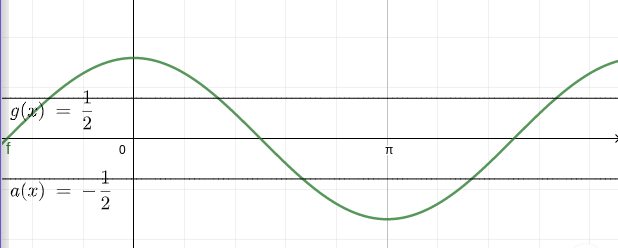
\includegraphics[width=0.4\linewidth]{img/cosine.png}
	\caption{$ \cos(x) $}
\end{figure}
Veamos que en los únicos lugares donde se interseca es en $ \theta = \dfrac{\pi}{3} $, y luego hasta $ \dfrac{2\pi}{3} $, pero dentro de este intervalo su valor absoluto es a lo más $ \dfrac{1}{2} $, lo mismo ocurre con $ \dfrac{4\pi}{3} $ y $ \dfrac{5\pi}{3}  $.\\

Por lo tanto, el conjunto de vectores que solucionan este problema es 
\[ \left\lbrace \vec{x} \quad | \quad \vec{x} \text{ es un vector unitario } \quad \land \quad \theta \in \left[ \dfrac{\pi}{3}, \dfrac{2\pi}{3} \right] \cup \left[ \dfrac{4\pi}{3}, \dfrac{5\pi}{3} \right]  \right\rbrace \]

donde $ \theta $ es el ángulo formado entre $ \nabla T(1,1,1) $ y el vector $ \vec{x} $

% el profe aún no me constesta pero seguiré dejando este espacio en blanco por si lo necestamos



\end{document}
